\section{Materials and Methods}

\subsection{The Avida Digital Evolution Platform}

% -- Define digital organisms --
Avida is a study system wherein self-replicating computer programs (digital organisms) compete for space on a finite toroidal grid \citep{ofria_avida:_2009}.
Each digital organism is defined by a linear sequence of program instructions (its genome) and a set of virtual hardware components used to interpret and express those instructions. 
Genomes are expressed sequentially except when the execution of one instruction deterministically changes which instruction should be executed next (\textit{e.g.}, a ``jump'' instruction). 
Genomes are built using an instruction set that is both robust (\textit{i.e.}, any ordering of instructions is syntactically valid, though not necessarily meaningful) and Turing Complete (\textit{i.e.}, able to represent any computable function, though not necessarily in an efficient manner).
The instruction set includes operations for basic computations, flow control (\textit{e.g.}, conditional logic and looping), input, output, and self-replication.

% -- Define reproduction & mutation --
Organisms in Avida reproduce asexually by copying their genome instruction-by-instruction and then dividing. 
However, copy operations are imperfect and can result in single-instruction substitution mutations in an offspring's genome. 
For this work, we configured copy operations to err at a rate of one expected mutation for every 400 instructions copied (\textit{i.e.}, a per-instruction error rate of 0.0025).
We held individual genomes at a fixed length of 100 instructions; that is, we did not include insertion and deletion mutations. 
We used fixed-length genomes to control for treatment-specific conditions resulting in the evolution of substantially different genome sizes \citep{consequences_of_plasticity_supplemental_material_2021}\footnote{
We repeated our experiments without genome size restrictions and observed qualitatively similar results (see supplemental material, \citealt{consequences_of_plasticity_supplemental_material_2021}).
}, which could, on its own, drive differences in evolutionary outcomes among experimental treatments.
When an organism divides in Avida, its offspring is placed in a random location on the toroidal grid, replacing any previous occupant.
For this work, we used the default 60 by 60 grid size, which limits the maximum population size to 3600 organisms.
As such, improvements to the speed of self-replication are advantageous in the competition for space.

% -- Define fitness/metabolic rate/improving replication speed --
During evolution, organism replication rates improve in two ways: by improving genome efficiency (\textit{e.g.}, using a more compact encoding) or by accelerating the rate at which the genome is expressed (their ``metabolic rate'').
An organism's metabolic rate determines the speed at which it executes instructions in its genome.
Initially, an organism's metabolic rate is proportional to the length of its genome, but that rate is adjusted as it completes designated tasks, such as performing Boolean logic computations \citep{ofria_avida:_2009}.
In this way, we can reward or punish particular phenotypic traits. 

\subsubsection{Phenotypic plasticity in Avida}

% -- Phenotypes & Phenotypic plasticity --
%   - What is a phenotype in Avida?
In this work, we measure a digital organism's phenotype as the set of Boolean logic functions that it performs in a given environment.
Sensory instructions in the Avida instruction set allow organisms to detect how performing a particular logic function would affect their metabolic rate (see supplemental material for more details, \citealt{consequences_of_plasticity_supplemental_material_2021}). 
We define a phenotypically plastic organism as one that uses sensory information to alter which logic functions it performs based on the environment.

% -- Adaptive plasticity & non-adaptive plasticity --
Phenotypic plasticity in Avida can be adaptive or non-adaptive for a given set of environments.
Adaptive plasticity shifts net task expression closer to the optimum for the given environments.
Non-adaptive plasticity changes task expression in either a neutral or deleterious way. 
Optimal plasticity toggles tasks to always perfectly match the set of rewarded tasks for the given set of environments.

\subsection{Experimental design}
\label{chapter:consequences-of-plasticity:sec:methods:experiment}

\begin{figure}[ht!]
    \centering
    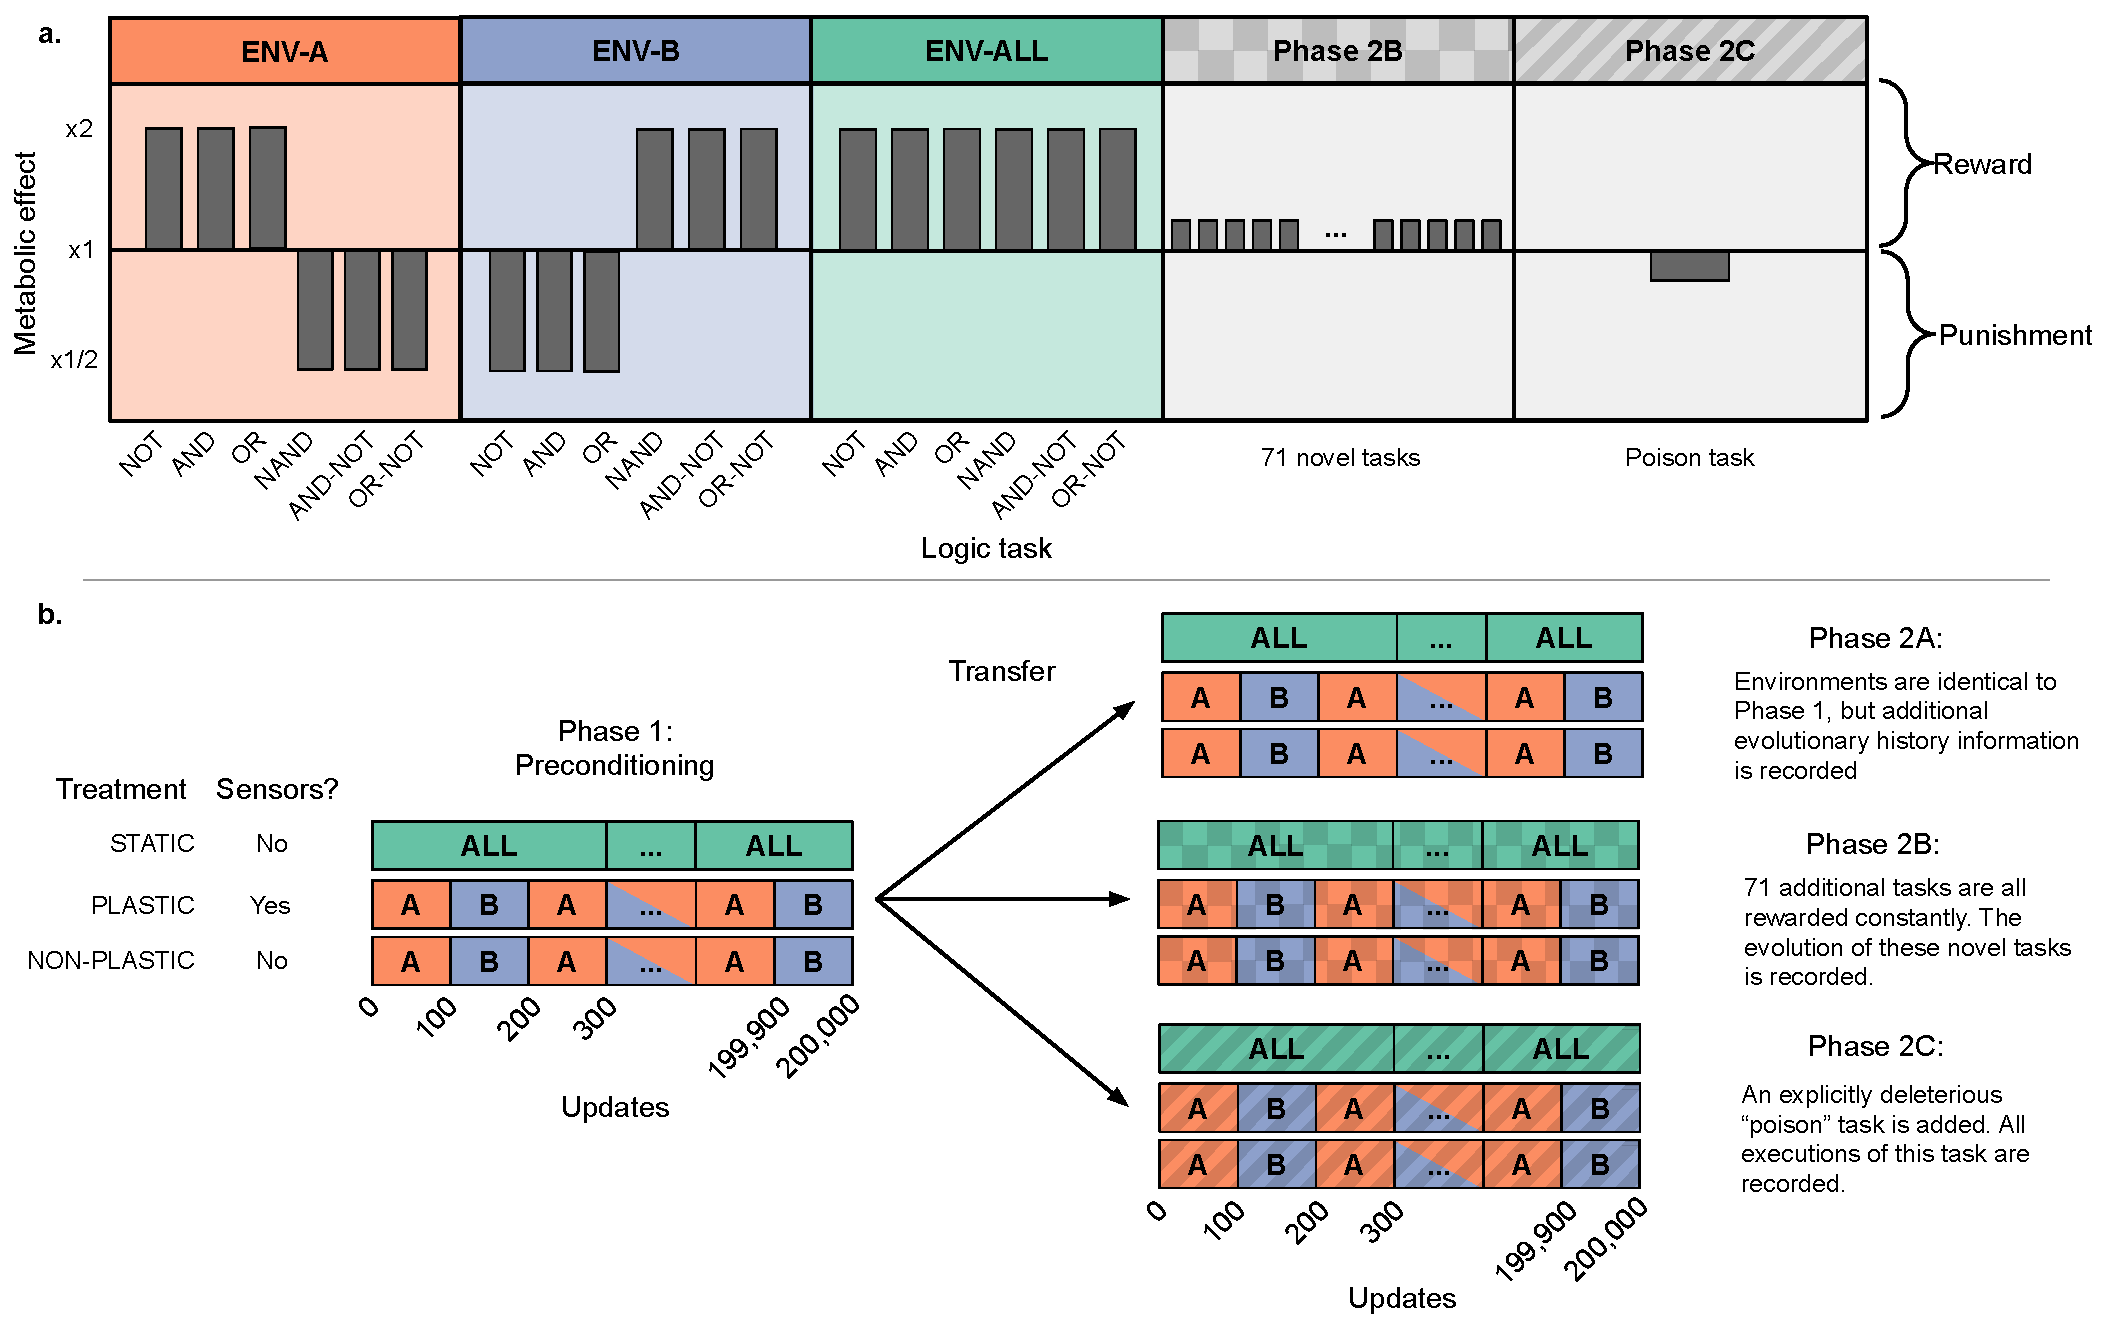
\includegraphics[width=1\textwidth]{chapters/03-evolutionary-consequences-of-plasticity/media/experimental-design.pdf}
    \caption{\small
    \textbf{Overview of experimental design.}
    The first three plots in panel (a) show the environments used in every experiment and whether they reward or punish each base task. 
    Additionally, the last two subplots in (a) show the additional tasks added in phases 2B and 2C. 
    All novel tasks confer a 10\% metabolic reward, while executing the poisonous task causes a 10\% metabolic punishment (bars not drawn to size). 
    Panel (b) shows treatment differences and experiment phases. 
    Treatments are listed on the left, with each treatment consisting of an environment timeline and whether sensors are functional. 
    % This also shows Phase 1, the preconditioning phase.  
    We conducted three independent two-phase experiments, each described on the right.
    % We conducted experiments using three different second phases, as shown on the right. 
    Phases 2B and 2C are textured to match their task definitions in panel (a). 
    Phase one is repeated for \textit{each} experiment with 100 replicate populations per treatment per experiment. 
    For each replicate at the end of phase one, we used an organism of the abundant genotype to found the second phase population. 
    All STATIC and NON-PLASTIC populations move on to phase two, but PLASTIC populations only continue to the second phase if their most abundant genotype exhibits optimal plasticity. 
    Metrics are recorded only in phase two. 
    }
    \label{chapter:consequences-of-plasticity:fig:experimental-design}
\end{figure}

%%%%%%%%%%%%%%%%%%%%%%%%%%%%%%%%%%%%%%%%%%%%%%%%%
% OUTLINE
%%%%%%%%%%%%%%%%%%%%%%%%%%%%%%%%%%%%%%%%%%%%%%%%%
% Overview of experimental design
% - Focused around diagram
% Environment implementations
% Specifications for Phase 1
% specifications for Phase 2A
% specifications for Phase 2B
% specifications for Phase 2C
%%%%%%%%%%%%%%%%%%%%%%%%%%%%%%%%%%%%%%%%%%%%%%%%%

% -- Treatments --
We conducted three independent experiments using Avida to investigate how the evolution of adaptive plasticity influences evolutionary outcomes in fluctuating environments.
For each experiment, we compared the evolutionary outcomes of populations evolved under three treatments (Figure \ref{chapter:consequences-of-plasticity:fig:experimental-design}): 
(1) a \textbf{PLASTIC} treatment where the environment fluctuates, and digital organisms can use sensory instructions to differentiate between environmental states;
(2) a \textbf{NON-PLASTIC} treatment with identical environment fluctuations, but where sensory instructions are disabled;
and (3) a \textbf{STATIC} control where organisms evolve in a constant environment.

% -- Experiment phases --
Each experiment was divided into two phases that each lasted for 200,000 updates\footnote{
    One update in Avida is the amount of time required for the average organism to execute 30 instructions. 
    See \citep{ofria_avida:_2009} for more details.
} of evolution (Figure \ref{chapter:consequences-of-plasticity:fig:experimental-design}), which is approximately 30,000 to 40,000 generations.
In phase one of each experiment, we preconditioned populations to their treatment-specific conditions.
In phase two, we founded new populations with the evolved organisms from phase one and examined their subsequent evolution under given combinations of treatment and experimental conditions.
During phase two, we tracked each population's evolutionary history as well as saving the full final population.
Phase one was for pre-conditioning only; all comparisons between treatments were performed on phase two data.

\subsubsection{Environments}
\label{chapter:consequences-of-plasticity:sec:methods:experiment:environments}

% ----- ENVIRONMENTS -----
% traits_set_a <- c("not", "and", "or")
% traits_set_b <- c("nand", "ornot", "andnot")

% -- Environment definitions --
We constructed three experimental environments, abbreviated hereafter as ``ENV-A'', ``ENV-B'', and ``ENV-ALL''.
Figure \ref{chapter:consequences-of-plasticity:fig:experimental-design} describes these environments based on whether each of six Boolean logic tasks (NOT, NAND, AND, OR-NOT, OR, and AND-NOT) is rewarded or punished.
A rewarded task performed by an organism doubles their metabolic rate, allowing them to execute twice as many instructions in the same amount of time.
A punished task halves an organism's metabolic rate. 

% -- Treatment-specific environment details --
In both the PLASTIC and NON-PLASTIC conditions, the environment cycles between equal-length periods of ENV-A and ENV-B.
Each of these periods persist for 100 updates (approximately 15 to 20 generations).
Thus, populations experience a total of 1,000 full periods of ENV-A interlaced with 1,000 full periods of ENV-B during each experimental phase.

% -- Sensory instructions + control flow and controlling the capacity for plasticity --
Organisms in the PLASTIC treatments differentiate between ENV-A and ENV-B by executing one of six sensory instructions, each associated with a particular logical task; these sensory instructions detect whether their associated task is currently rewarded or punished.
By using sensory information in combination with execution flow-control instructions, organisms can conditionally perform different logic tasks depending on the current environmental conditions.

\subsubsection{Experiment Phase 1 -- Environment preconditioning}
\label{chapter:consequences-of-plasticity:sec:methods:experiment:phase-one}

For each treatment, we founded 100 independent populations from a common ancestral strain capable only of self-replication.
At the end of phase one, we identified the most abundant (\textit{i.e.}, dominant) genotype and extracted an organism with that genotype from each replicate population to found a new population for phase two.

For the PLASTIC treatment, we measure plasticity by independently testing a given genotype in each of ENV-A and ENV-B.
We discard phase one populations if the dominant genotype does not exhibit optimal plasticity.
This approach ensures that measurements taken on PLASTIC-treatment populations during the second phase of each experiment reflect the evolutionary consequences of adaptive plasticity.

\subsubsection{Experiment Phase 2A -- Evolutionary change rate}
\label{chapter:consequences-of-plasticity:sec:methods:experiment:evolutionary-change-rate}

Phase 2A continued exactly as phase one, except we tracked the rates of evolutionary change in each of the PLASTIC-, NON-PLASTIC-, and STATIC-treatment populations. 
Specifically, we quantified evolutionary change rates using four metrics (each described in Table~\ref{chapter:consequences-of-plasticity:tab:metrics-definitions}):
(1) coalescence event count,
(2) mutation count, 
(3) phenotypic volatility,
and (4) mutational stability.
We additionally used knockout experiments to examine how the genetic architectures of organisms and their ancestors changed over time, measuring the architectural volatility (Table~\ref{chapter:consequences-of-plasticity:tab:metrics-definitions}) of evolved lineages.

\subsubsection{Experiment Phase 2B -- Novel task evolution}
\label{chapter:consequences-of-plasticity:sec:methods:experiment:novel-task-evolution}

Phase 2B extended the conditions of phase one by adding 71 novel Boolean logic tasks, which were always rewarded in all treatments \citep{ofria_avida:_2009}.
The original six phase one tasks (NOT, NAND, AND, OR-NOT, OR, and AND-NOT; hereafter called ``base'' tasks) continued to be rewarded or punished according to the particular treatment conditions.
An organism's metabolic rate was increased by \novelTraitsReward\ for each novel task that it performed (limited to one reward per task).
This reward provided a selective pressure to evolve these tasks, but their benefits did not overwhelm the 100\% metabolic rate increase conferred by rewarded base tasks. 
As such, populations in the PLASTIC and NON-PLASTIC treatments could not easily escape environmental fluctuations by abandoning the fluctuating base tasks.

During this experiment, we tracked the extent to which populations evolving under each treatment were capable of acquiring and retaining novel tasks.  
Specifically, we used three metrics (each described in Table~\ref{chapter:consequences-of-plasticity:tab:metrics-definitions}):
(1) final novel task count,     
(2) novel task discovery,    
and (3) novel task loss. 

\subsubsection{Experiment Phase 2C -- Deleterious instruction accumulation}
\label{chapter:consequences-of-plasticity:sec:methods:experiment:deleterious-instruction-accumulation}

Phase 2C extended the instruction set of phase one with a \code{poison} instruction.
When an organism executes a \code{poison} instruction, it performs a ``poisonous'' task, which reduces the organism's metabolic rate (and thus reproductive success) but does not otherwise alter the organism's function.
We imposed a 10\% penalty each time an organism performed the poisonous task, making the \code{poison} instruction explicitly deleterious to execute.
We did not limit the number of times that an organism could perform the poisonous task, and as such, organisms could perform the poisonous task as many times as they executed the \code{poison} instruction. 

We tracked the number of times each organism along the dominant lineage performed the poisonous task.
Specifically, we used two metrics (each described in Table~\ref{chapter:consequences-of-plasticity:tab:metrics-definitions}):
(1) final poisonous task count,
and (2) poisonous task acquisition.

\subsection{Experimental analyses}

%%%%%%%%%%%%%%%%%%% METRIC DEFINITIONS (used in table) %%%%%%%%%%%%%%%%%%%
\newcommand{\SweepsMetricName}{
Coalescence event count
}
\newcommand{\SweepsMetricDesc}{
Number of coalescence events that have occurred, which indicates the frequency of selective sweeps in the population.
}

\newcommand{\MutationCountMetricName}{
Mutation count
}
\newcommand{\MutationCountMetricDesc}{
Sum of all mutations that have occurred along a lineage.
}

\newcommand{\PhenotypicVolatilityMetricName}{
Phenotypic volatility
}
\newcommand{\PhenotypicVolatilityMetricDesc}{
Number of instances where parent and offspring phenotypic profiles do not match along a lineage.
Phenotypic volatility as defined here indicates the rate at which accumulated genetic changes actually change the phenotype along a lineage.
}

\newcommand{\MutationalStabilityMetricName}{
Mutational stability
}
\newcommand{\MutationalStabilityMetricDesc}{
Proportion of mutated offspring along a lineage whose phenotypic profile matches that of their parent. 
}

\newcommand{\GenotypicFidelityMetricName}{
Genotypic fidelity
}
\newcommand{\GenotypicFidelityMetricDesc}{
Frequency that an offspring's genotype is identical to its parent's genotype along a given lineage.
}

\newcommand{\PhenotypicFidelityMetricName}{
Phenotypic fidelity
}
\newcommand{\PhenotypicFidelityMetricDesc}{
Frequency that an offspring's phenotypic profile is identical to its parent's phenotypic profile along a given lineage.
}

\newcommand{\TaskPerformanceMetricName}{
Final novel task count
}
\newcommand{\TaskPerformanceMetricDesc}{
Count of unique novel tasks performed by the representative organism in a final population from experiment \hyperref[chapter:consequences-of-plasticity:sec:methods:experiment:novel-task-evolution]{phase 2B}. 
This metric can range from 0 to 71 and measures the level of exploitation of the fitness landscape (\textit{i.e.}, the mapping between genetic space and phenotype space) at a given point in time.
}

\newcommand{\TaskDiscoveryMetricName}{
Novel task discovery
}
\newcommand{\TaskDiscoveryMetricDesc}{
Number of unique novel tasks ever performed along a given lineage in experimental \hyperref[chapter:consequences-of-plasticity:sec:methods:experiment:novel-task-evolution]{phase 2B}, even if a task is later lost.
This metric can range from 0 to 71 and measures a given lineage's level of exploration of the fitness landscape.
}

\newcommand{\TaskLossMetricName}{
Novel task loss
}
\newcommand{\TaskLossMetricDesc}{
Number of instances along a given lineage from experimental \hyperref[chapter:consequences-of-plasticity:sec:methods:experiment:novel-task-evolution]{phase 2B} where a novel task is performed by a parent but not its offspring. 
This metric measures how often a given lineage fails to retain evolved traits over time.
}

\newcommand{\FinalPoisonMetricName}{
Final poisonous task count
}
\newcommand{\FinalPoisonMetricDesc}{
Number of times the poisonous task is performed by the representative organism from a final population from experiment \hyperref[chapter:consequences-of-plasticity:sec:methods:experiment:deleterious-instruction-accumulation]{phase 2C}.
}

\newcommand{\LineagePoisonMetricName}{
Poisonous task acquisition count
}
\newcommand{\LineagePoisonMetricDesc}{
Number of instances along a given lineage where a mutation causes an offspring perform the poisonous task more times than its parent. 
}

\newcommand{\ArchitectureVolatilityMetricName}{
Architectural volatility
}
\newcommand{\ArchitectureVolatilityMetricDesc}{
The average number of mutations that cause a change in the function of loci along a lineage. 
%Loci function is denoted as the combination of task machinery, plasticity machinery, vestigial machinery for both ENV-A and ENV-B tasks, as well as replication and required machinery. 
}


%%%%%%%%%%%%%%%%%%% TABLE %%%%%%%%%%%%%%%%%%%

\newcommand*{\thead}[1]{\multicolumn{1}{c}{\bfseries #1}}

\setlength{\tabcolsep}{12pt}
\renewcommand{\arraystretch}{1.1}
\begin{table}[ht!]
    \centering
    
    \rowcolors{2}{gray!25}{white}
    \begin{tabularx}{\linewidth}{lX} % p{10cm}
        \rowcolor{gray!50}
        \hline 
        \thead{Metric} & \thead{Description}   \\
        \hline
        \SweepsMetricName & \SweepsMetricDesc \\
        \MutationCountMetricName & \MutationCountMetricDesc \\
        \PhenotypicVolatilityMetricName & \PhenotypicVolatilityMetricDesc \\
        \MutationalStabilityMetricName & \MutationalStabilityMetricDesc \\
        \ArchitectureVolatilityMetricName & \ArchitectureVolatilityMetricDesc \\
        \TaskPerformanceMetricName & \TaskPerformanceMetricDesc \\
        \TaskDiscoveryMetricName & \TaskDiscoveryMetricDesc \\
        \TaskLossMetricName & \TaskLossMetricDesc \\
        \FinalPoisonMetricName & \FinalPoisonMetricDesc \\
        \LineagePoisonMetricName & \LineagePoisonMetricDesc \\
        \hline
    \end{tabularx}
    
    \caption{\textbf{Metric descriptions.}}
    \label{chapter:consequences-of-plasticity:tab:metrics-definitions}
\end{table}
\renewcommand{\arraystretch}{1.0}




% naive environment = what organism experiencing
% alternative environment = what organism is not currently experiencing

% - How we extracted representative lineages -
For each of our experiments, we tracked and analyzed the phylogenetic histories of evolving populations during phase two. 
For each replicate, we identified an organism with the most abundant genotype in the final evolved population, and we used it as a representative organism for further analysis.
We then isolated the lineage from the founding organism to the representative organism, which we used as the representative lineage for further analysis.
We manually inspected evolved phylogenies and found no evidence that any of our experimental treatments supported long-term coexistence. 
As such, each of the representative lineages reflect the majority of evolutionary history from a given population at the end of our experiment.

% -- PHENOTYPIC PROFILE --
Some of our metrics required us to measure genotype-by-environment interactions.
Importantly, in the fluctuating environments, we needed to differentiate phenotypic changes that were caused by mutations from those that were caused by environmental changes.
To accomplish this, we produced organisms with the focal genotype, measured their phenotype in each environment, and aggregated the resulting phenotypes to create a \textit{phenotypic profile}. 
Although organisms with different genotypes may express the same set of tasks across environments, their phenotypic profiles may not necessarily be the same.
For example, an organism that expresses NOT in ENV-A and NAND in ENV-B has a distinct phenotypic profile from one that expresses NAND in ENV-A and NOT in ENV-B.

% -- KNOCKOUT EXPERIMENTS --
For an individual organism, we can perform knockout experiments to identify which instructions are responsible for producing a given phenotypic outcome.
To perform a knockout, we duplicate the organism, replacing a single instruction with an inert ``no-operation'' instruction.
We then identify any phenotypic changes by contrasting the execution results of the ``knockout'' organism and the original.
Such changes provide evidence of the role that the original instruction must have played in the genome.
For example, when an organism performs the NAND task but loses it when an instruction is knocked out, we categorize that instruction as part of the NAND task machinery.
We use knockout experiments to characterize the role of each instruction in the genomes of every organism along all study lineages, revealing how genetic architectures change over time.

\subsection{Statistical analyses}

Across all of our experiments, we differentiated between sample distributions using non-parametric statistical tests.
For each major analysis, we first performed a Kruskal-Wallis test \citep{kruskal_use_1952} to 
determine if there were significant differences in results from the PLASTIC, NON-PLASTIC, and STATIC treatments (significance level $\alpha=0.05$).
If so, we applied a Wilcoxon rank-sum test \citep{kotz_individual_1992} to distinguish between pairs of treatments.
We applied Bonferroni corrections for multiple comparisons \citep{rice_analyzing_1989} where appropriate.

\subsection{Software availability}

We conducted our experiments using a modified version of the Avida software, which is open source and freely available on \href{https://github.com/amlalejini/evolutionary-consequences-of-plasticity}{GitHub} \citep{consequences_of_plasticity_supplemental_material_2021}.
We used Python for data processing, and we conducted all statistical analyses using R version 4 \citep{r_core_team_r_v4}.
We used the tidyverse collection of R packages \citep{r_tidyverse_2019} to wrangle data, and we used the following R packages for analysis, graphing, and visualization: 
ggplot2 \citep{R-ggplot2}, 
cowplot \citep{R-cowplot}, 
Color Brewer \citep{harrower_colorbrewerorg_2003,R-Brewer_2014}, 
rstatix \citep{R-rstatix},
ggsignif \citep{R-ggsignif},
scales \citep{R-scales},
Hmisc \citep{R-Hmisc}, 
fmsb \citep{R-fmsb}, 
and boot \citep{R-boot}.
We used R markdown \citep{rmarkdown} and bookdown \citep{R-bookdown} to generate web-enabled supplemental material.
All of the source code for our experiments and analyses, including guides for replication and configuration files, can be found in our supplemental material, which is hosted on \href{https://github.com/amlalejini/evolutionary-consequences-of-plasticity}{GitHub} \citep{consequences_of_plasticity_supplemental_material_2021}.
Additionally, our experimental data is available on the Open Science Framework at \url{https://osf.io/sav2c/} \citep{consequences_of_plasticity_osf_data}.